\chapter{Einleitung, Motivation - motivation}

Hier auch erwähnen in welchem Kameramodell wir uns befinden (LITERATUR FINDEN DIE NICHT HZ IST!!)\\
Generelle kleine einleitung über kamerakalibrierung und was das genau ist (NICHT VIEL!!)

Kameramodellbeschreibung geometrisch in \cite{Jianzhong}\\

Ziel ist es auch bestimmte unklarheiten in der Literatur wie Einheiten in rechnungen wie fundamental und essentielle matrix aus der welt zu schaffen.\\

expliziet darauf eingehen, was es bedeutet zwei gleiche und zwei unterschiedliche Resolutions der Kameras zu besitzen gerade in Bezug auf die Ermittlung von F und E und der Szenenrekonstruktion(LITERATUR FINDEN DIE NICHT HZ IST!!)\\

Erwähnen mit was alles gearbeitet wurde (mathematica, Geogebra, Matlab, Unity(nur wenig))


	\begin{minipage}{\linewidth}
	\centering
	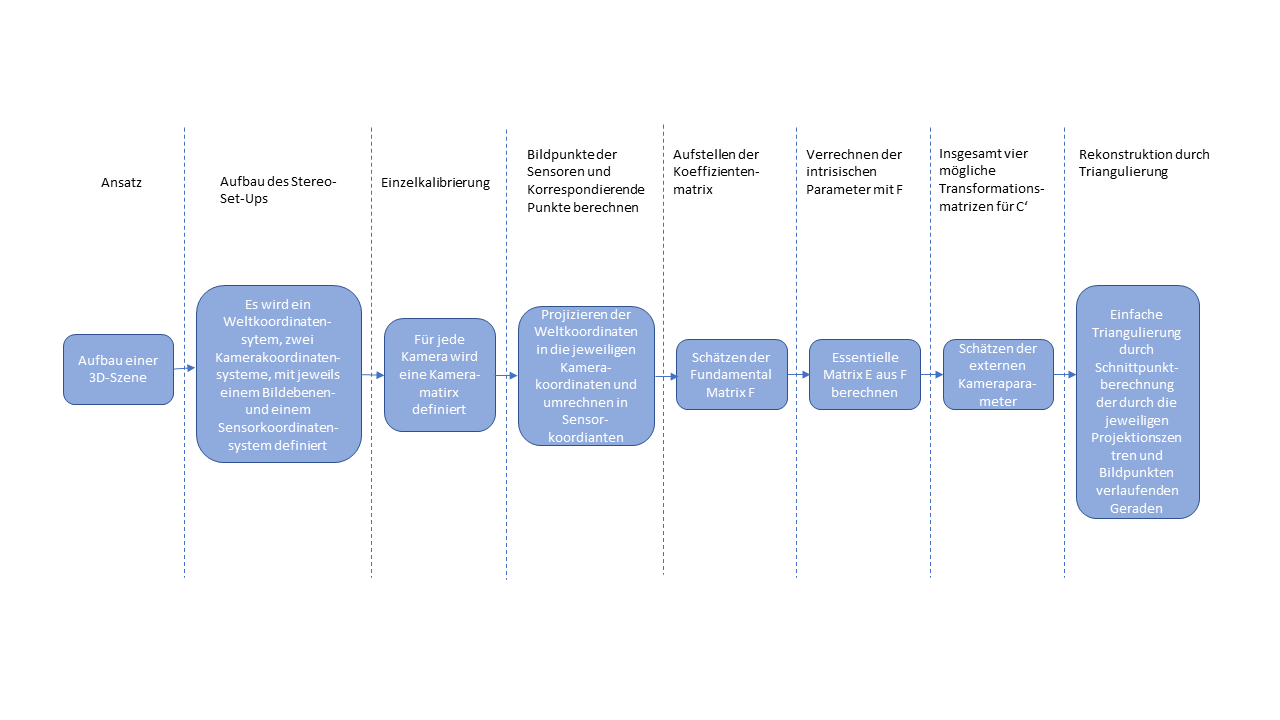
\includegraphics[width=1.\linewidth]{images/ArbeitsProzessMinimal.png}
	\captionof{figure}{Arbeitsprozesse der Stereoanalyse bei Verwendung von eigens erstellten synthetischen Bilddaten}
\end{minipage}\\ \\


	\begin{minipage}{\linewidth}
	\centering
	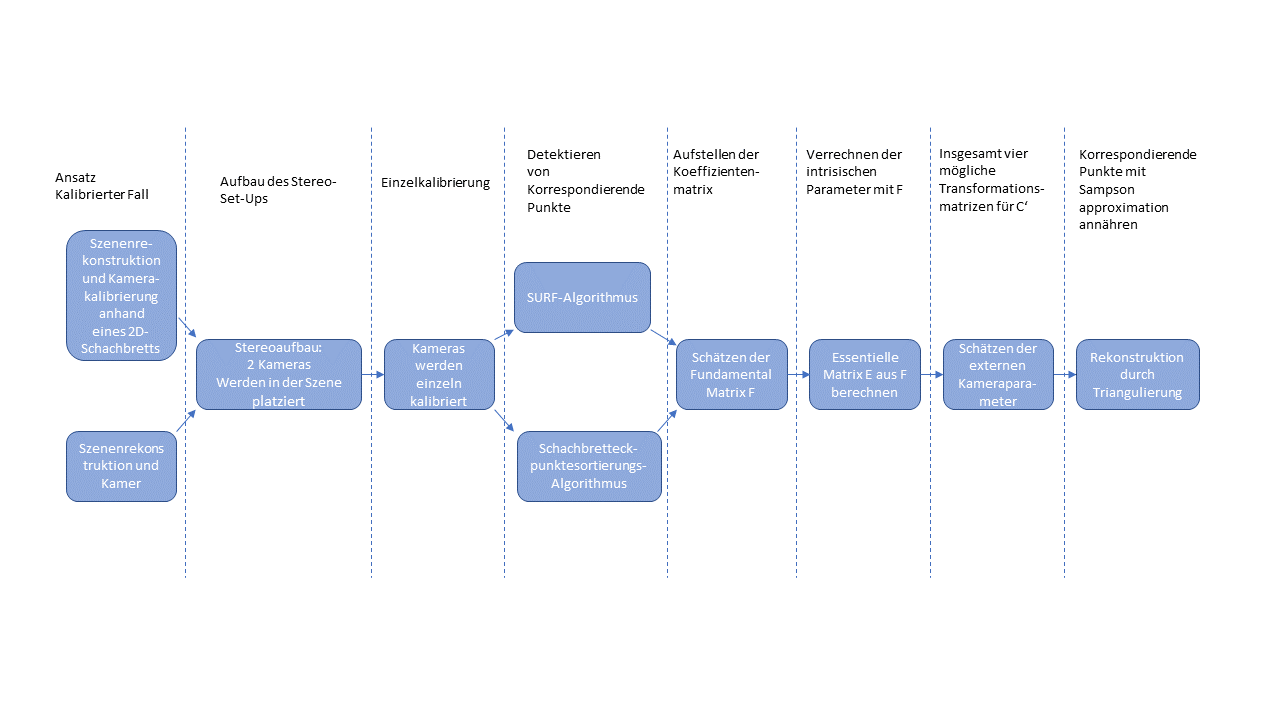
\includegraphics[width=1.\linewidth]{images/ArbeitsProzessReal.png}
	\captionof{figure}{Arbeitsprozesse der Stereoanalyse bei Verwendung von realen Bilddaten}
\end{minipage}\\ \\

